\subsection{Normalized Mutual Information evolution}

	\subsubsection{NMI evolution over number of clusters for 2 zernike mode related datasets}
		\begin{figure*}[ht!]
			\centering
			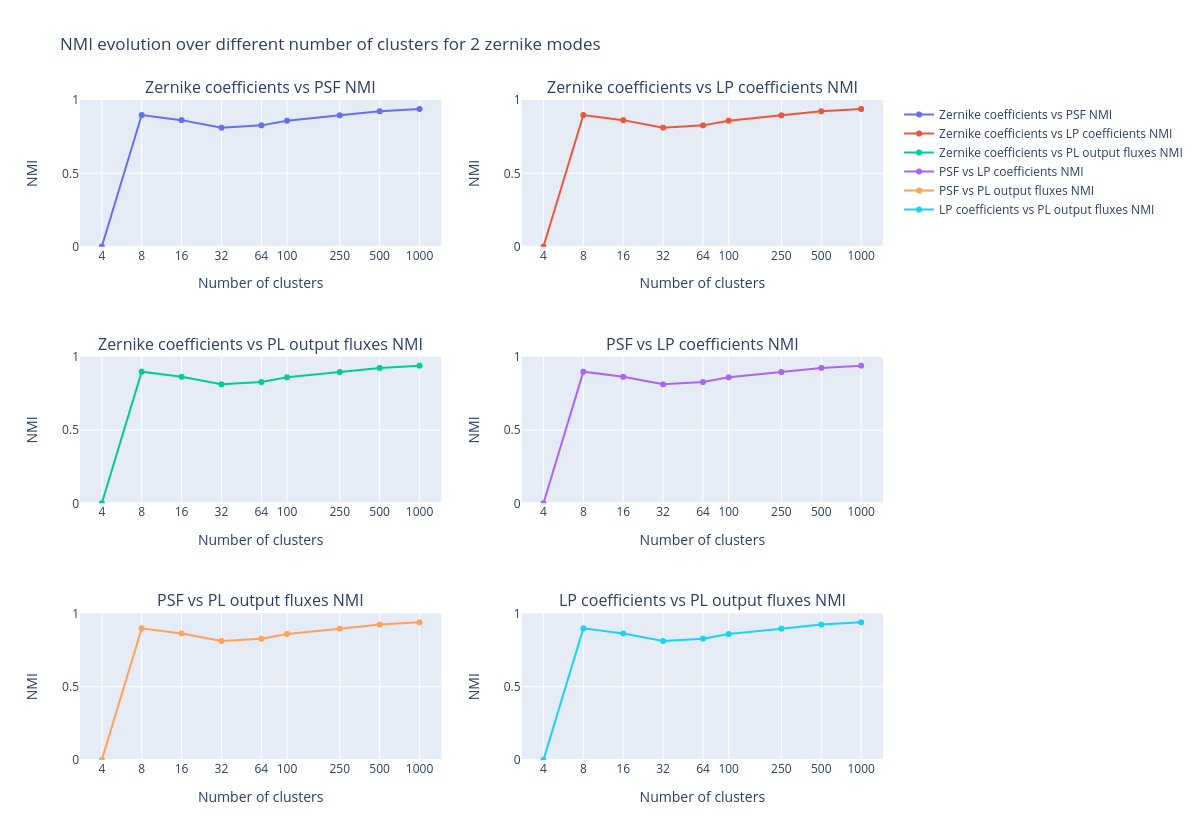
\includegraphics[width=0.9\textwidth]{nmia-nmievolutionover2.png}
		\end{figure*}
		\FloatBarrier
		
	\subsubsection{NMI evolution over number of clusters for 5 zernike mode related datasets}
		\begin{figure*}[ht!]
			\centering
			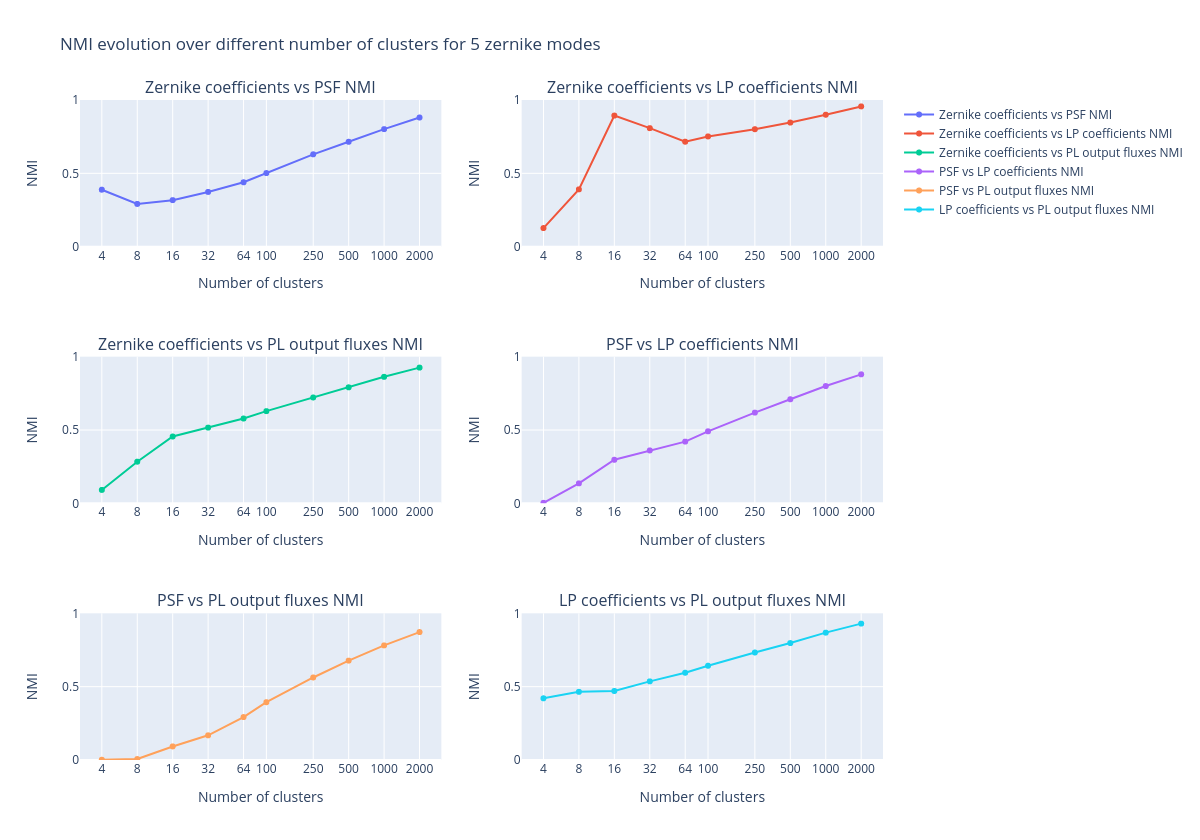
\includegraphics[width=0.9\textwidth]{nmia-nmievolutionover5.png}
		\end{figure*}
		\FloatBarrier
		
	\subsubsection{NMI evolution over number of clusters for 9 zernike mode related datasets}
		\begin{figure*}[ht!]
			\centering
			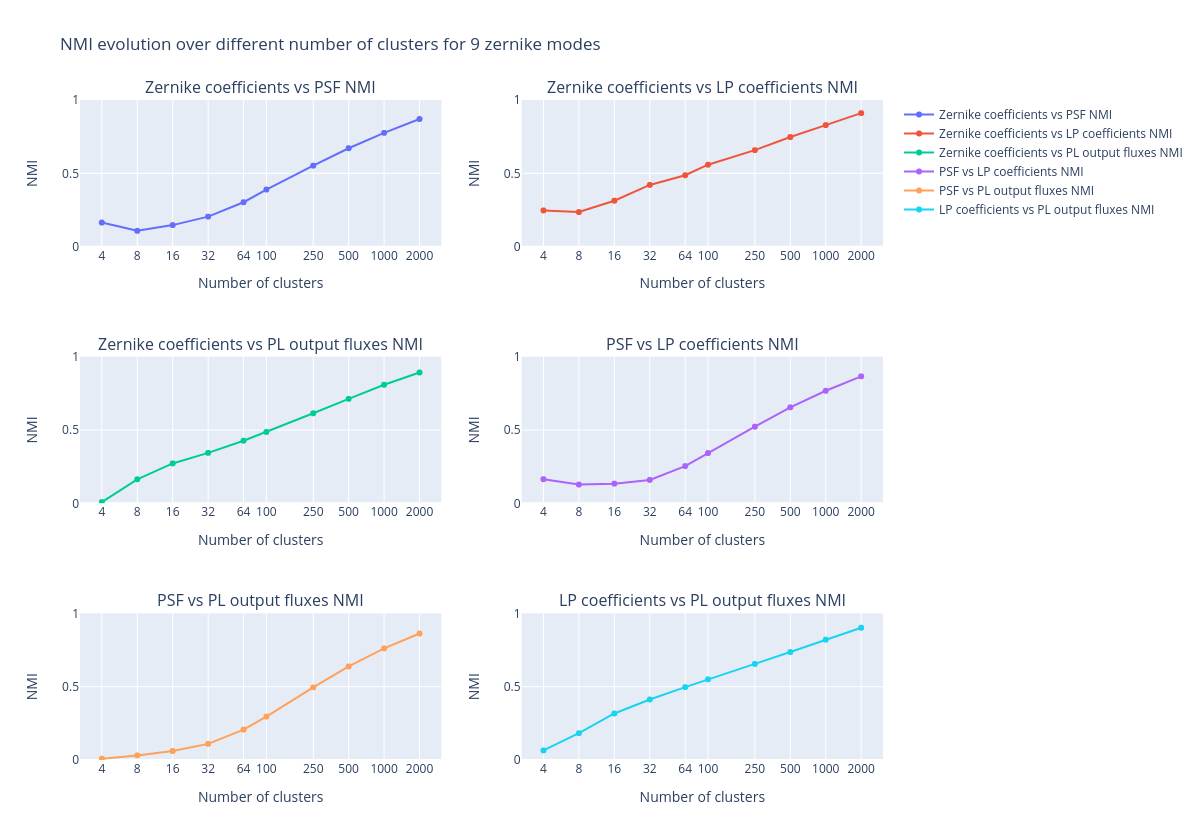
\includegraphics[width=0.9\textwidth]{nmia-nmievolutionover9.png}
		\end{figure*}
		\FloatBarrier
		
	\subsubsection{NMI evolution over number of clusters for 14 zernike mode related datasets}
		\begin{figure*}[ht!]
			\centering
			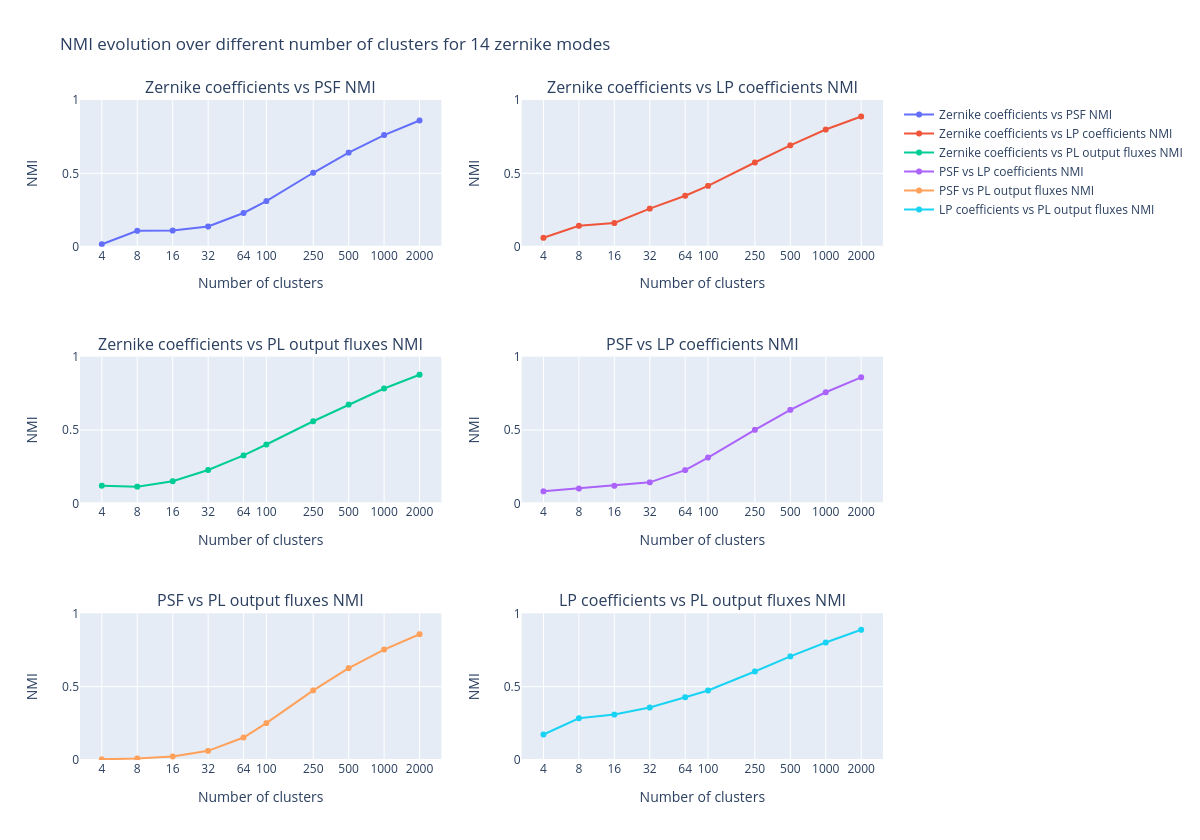
\includegraphics[width=0.9\textwidth]{nmia-nmievolutionover14.png}
		\end{figure*}
		\FloatBarrier
		
	\subsubsection{NMI evolution over number of clusters for 20 zernike mode related datasets}
		\begin{figure*}[ht!]
			\centering
			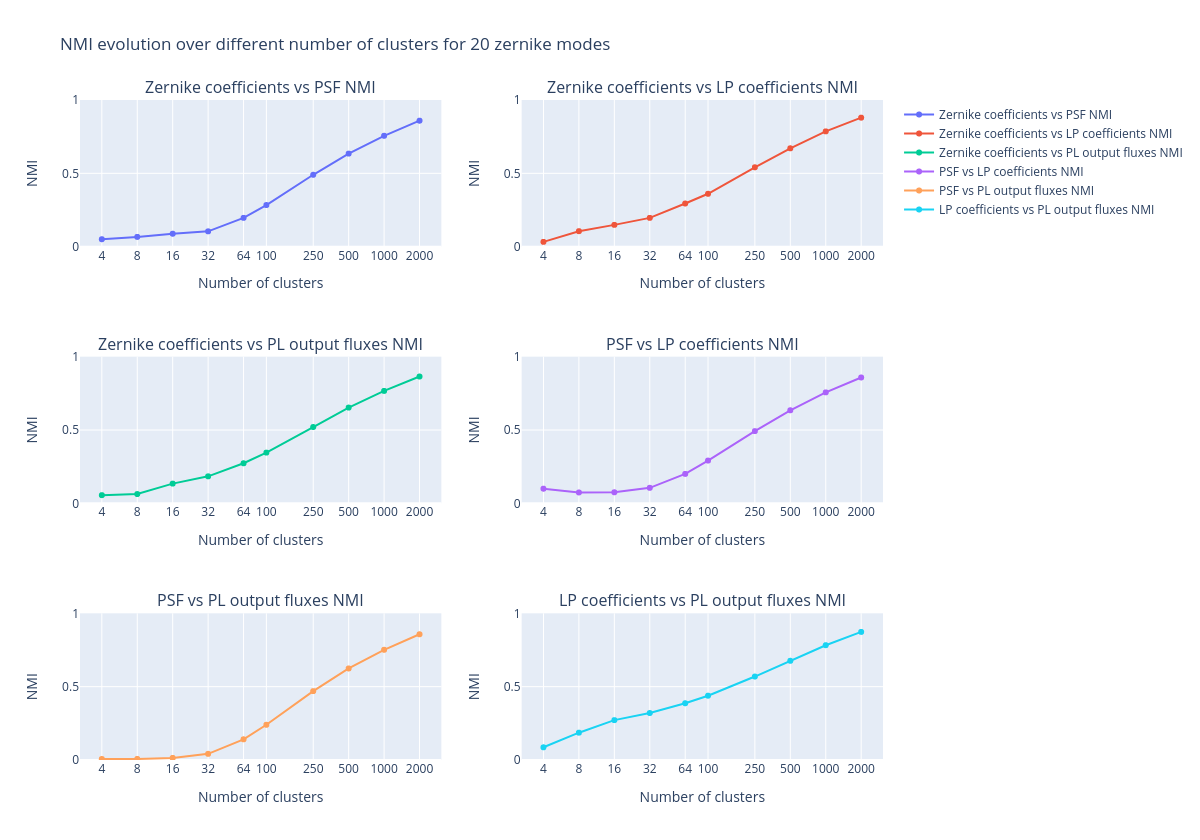
\includegraphics[width=0.9\textwidth]{nmia-nmievolutionover20.png}
		\end{figure*}
		\FloatBarrier
		
		
	\subsubsection{NMI evolution over number of zernike modes}
	
	\begin{figure*}[ht!]
			\centering
			\subfloat[NMI evolution over number of clusters for Zernike coefficients vs PSF]{%
				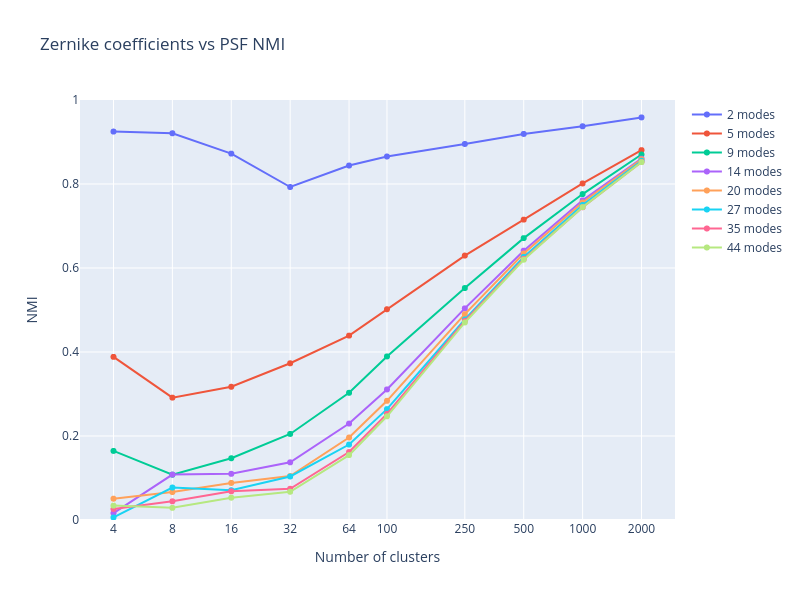
\includegraphics[width=0.45\textwidth]{nmia-zernikecoefficientsvspsfnmi.png}}
			\hspace{\fill}
			\subfloat[NMI evolution over number of clusters for Zernike coefficients vs LP coefficients]{%
				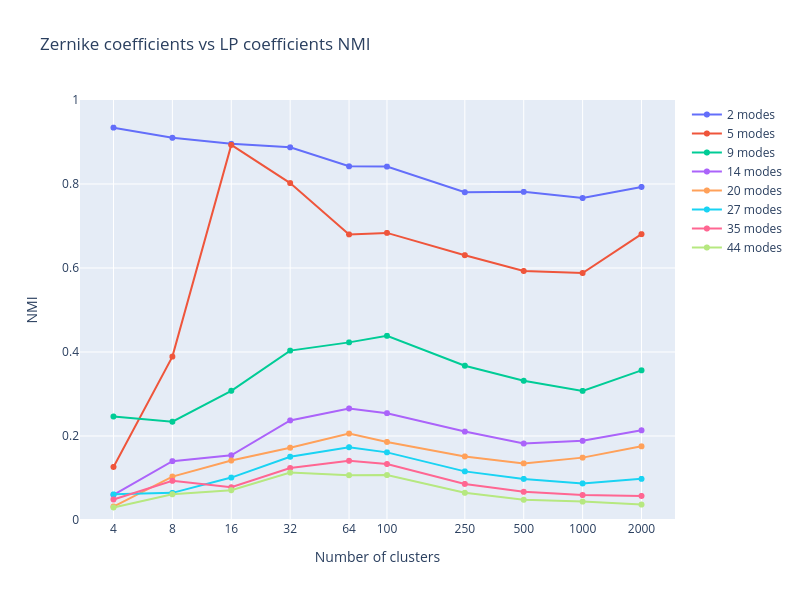
\includegraphics[width=0.45\textwidth]{nmia-zernikecoefficientsvslpcoefficientsnmi.png}}
			\\
			\subfloat[NMI evolution over number of clusters for Zernike coefficients vs PL output fluxes]{%
				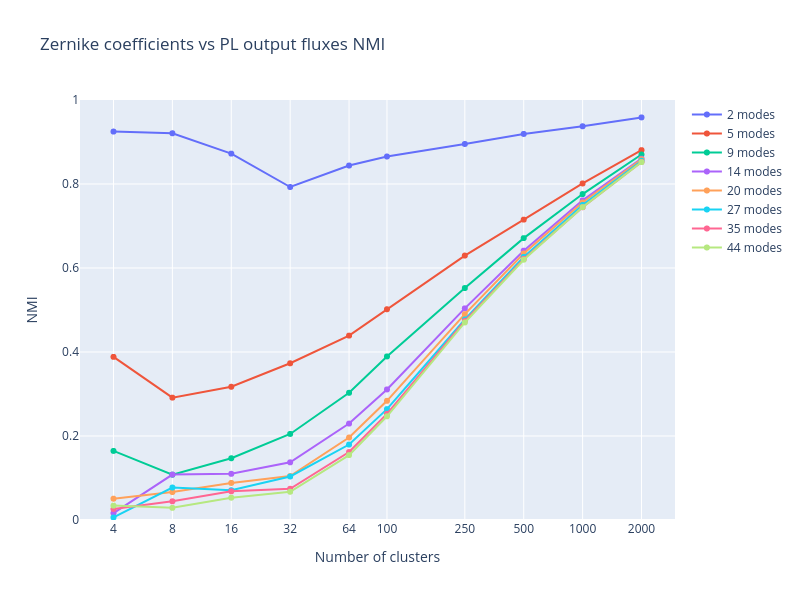
\includegraphics[width=0.45\textwidth]{nmia-zernikecoefficientsvsploutputfluxesnmi.png}}
			\hspace{\fill}
			\subfloat[NMI evolution over number of clusters for PSF vs LP coefficients]{%
				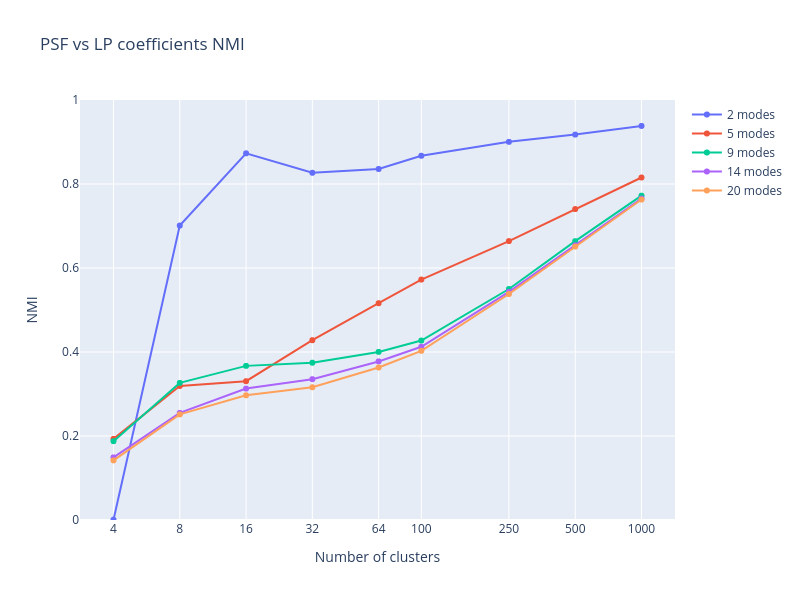
\includegraphics[width=0.45\textwidth]{nmia-psfvslpcoefficientsnmi.png}}
			\\
			\subfloat[NMI evolution over number of clusters for PSF vs PL output fluxes]{%
				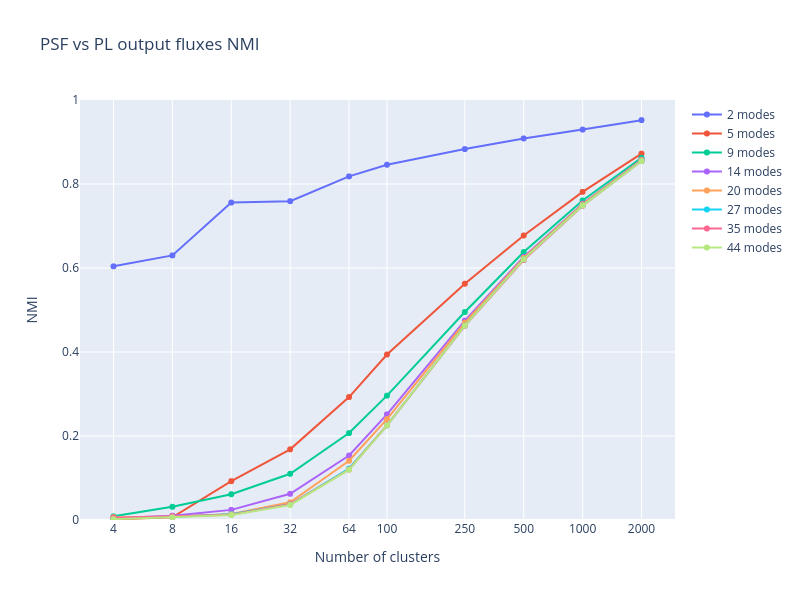
\includegraphics[width=0.45\textwidth]{nmia-psfvsploutputfluxesnmi.png}}
			\hspace{\fill}
			\subfloat[NMI evolution over number of clusters for LP coefficients vs PL output fluxes]{%
				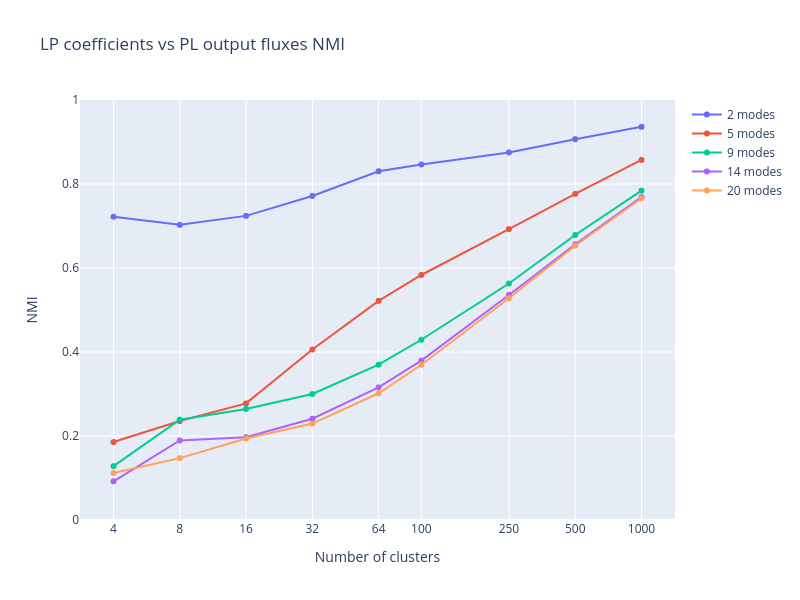
\includegraphics[width=0.45\textwidth]{nmia-lpcoefficientsvsploutputfluxesnmi.png}}
		\end{figure*}